% fig2_world.tex —— 图 2（建模世界）源文件。standalone 编译：
%   pdflatex fig2_world.tex
% 2026-11-27 重画：真实 10x10 格、100 台终端（一格一台）、盘半径 3 格；
% 两类终端用屏幕填充区分（sky-visible 亮屏 / sky-blind 白屏）；多跳上行路线按相邻格绘制。
% 环形网格：对边相邻，图上按展开画，图注说明。
\documentclass[border=4pt]{standalone}
\usepackage[T1]{fontenc}
\usepackage{amsmath}
\usepackage{xcolor}
\usepackage{tikz}
\usetikzlibrary{arrows.meta,calc}

\definecolor{cOurs}{RGB}{196,30,58}
\definecolor{cnblue}{RGB}{31,56,100}
\definecolor{cnteal}{RGB}{46,139,139}
\definecolor{cnpale}{RGB}{226,240,240}

% 终端图标：屏幕 0.62x0.46 格，底座。
\newcommand{\term}[3]{%
  \begin{scope}[shift={(#1,#2)}]
    \fill[#3] (-0.31,0.03) rectangle (0.31,0.49);
    \draw[cnblue!85,line width=0.5pt] (-0.31,0.03) rectangle (0.31,0.49);
    \draw[cnblue!85,line width=0.5pt] (0,0.03) -- (0,-0.06);
    \draw[cnblue!85,line width=0.5pt] (-0.17,-0.06) -- (0.17,-0.06);
  \end{scope}}
\newcommand{\dead}[2]{%
  \begin{scope}[shift={(#1,#2)}]
    \draw[cOurs,line width=0.8pt] (-0.36,-0.10) -- (0.36,0.52);
    \draw[cOurs,line width=0.8pt] (-0.36,0.52) -- (0.36,-0.10);
  \end{scope}}

\begin{document}
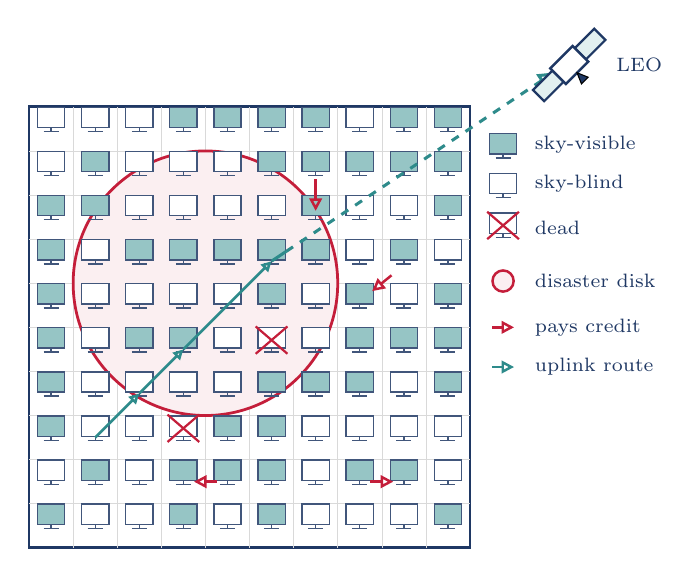
\begin{tikzpicture}[x=0.56cm,y=0.56cm,font=\sffamily]

% ---- 场地与网格（10x10，50 m 格）----
\draw[cnblue,line width=1pt] (0,0) rectangle (10,10);
\foreach \i in {1,...,9}{
  \draw[gray!30,line width=0.2pt] (\i,0) -- (\i,10);
  \draw[gray!30,line width=0.2pt] (0,\i) -- (10,\i);}

% ---- 灾盘：r = 3 格 = 150 m ----
\fill[cOurs!7] (4,6) circle (3);
\draw[cOurs,line width=1pt] (4,6) circle (3);

% ---- 100 台终端（一格一台）----
\term{0.5}{9.5}{white}
\term{1.5}{9.5}{white}
\term{2.5}{9.5}{white}
\term{3.5}{9.5}{cnteal!50}
\term{4.5}{9.5}{cnteal!50}
\term{5.5}{9.5}{cnteal!50}
\term{6.5}{9.5}{cnteal!50}
\term{7.5}{9.5}{white}
\term{8.5}{9.5}{cnteal!50}
\term{9.5}{9.5}{cnteal!50}
\term{0.5}{8.5}{white}
\term{1.5}{8.5}{cnteal!50}
\term{2.5}{8.5}{white}
\term{3.5}{8.5}{white}
\term{4.5}{8.5}{white}
\term{5.5}{8.5}{cnteal!50}
\term{6.5}{8.5}{cnteal!50}
\term{7.5}{8.5}{cnteal!50}
\term{8.5}{8.5}{cnteal!50}
\term{9.5}{8.5}{cnteal!50}
\term{0.5}{7.5}{cnteal!50}
\term{1.5}{7.5}{cnteal!50}
\term{2.5}{7.5}{white}
\term{3.5}{7.5}{white}
\term{4.5}{7.5}{white}
\term{5.5}{7.5}{white}
\term{6.5}{7.5}{cnteal!50}
\term{7.5}{7.5}{white}
\term{8.5}{7.5}{white}
\term{9.5}{7.5}{cnteal!50}
\term{0.5}{6.5}{cnteal!50}
\term{1.5}{6.5}{white}
\term{2.5}{6.5}{cnteal!50}
\term{3.5}{6.5}{cnteal!50}
\term{4.5}{6.5}{cnteal!50}
\term{5.5}{6.5}{cnteal!50}
\term{6.5}{6.5}{cnteal!50}
\term{7.5}{6.5}{white}
\term{8.5}{6.5}{cnteal!50}
\term{9.5}{6.5}{white}
\term{0.5}{5.5}{cnteal!50}
\term{1.5}{5.5}{white}
\term{2.5}{5.5}{white}
\term{3.5}{5.5}{white}
\term{4.5}{5.5}{white}
\term{5.5}{5.5}{cnteal!50}
\term{6.5}{5.5}{white}
\term{7.5}{5.5}{cnteal!50}
\term{8.5}{5.5}{white}
\term{9.5}{5.5}{cnteal!50}
\term{0.5}{4.5}{cnteal!50}
\term{1.5}{4.5}{white}
\term{2.5}{4.5}{cnteal!50}
\term{3.5}{4.5}{cnteal!50}
\term{4.5}{4.5}{white}
\term{5.5}{4.5}{white}\dead{5.5}{4.5}
\term{6.5}{4.5}{white}
\term{7.5}{4.5}{cnteal!50}
\term{8.5}{4.5}{cnteal!50}
\term{9.5}{4.5}{cnteal!50}
\term{0.5}{3.5}{cnteal!50}
\term{1.5}{3.5}{white}
\term{2.5}{3.5}{white}
\term{3.5}{3.5}{white}
\term{4.5}{3.5}{white}
\term{5.5}{3.5}{cnteal!50}
\term{6.5}{3.5}{cnteal!50}
\term{7.5}{3.5}{cnteal!50}
\term{8.5}{3.5}{white}
\term{9.5}{3.5}{cnteal!50}
\term{0.5}{2.5}{cnteal!50}
\term{1.5}{2.5}{white}
\term{2.5}{2.5}{white}
\term{3.5}{2.5}{white}\dead{3.5}{2.5}
\term{4.5}{2.5}{cnteal!50}
\term{5.5}{2.5}{cnteal!50}
\term{6.5}{2.5}{white}
\term{7.5}{2.5}{white}
\term{8.5}{2.5}{white}
\term{9.5}{2.5}{white}
\term{0.5}{1.5}{white}
\term{1.5}{1.5}{cnteal!50}
\term{2.5}{1.5}{white}
\term{3.5}{1.5}{cnteal!50}
\term{4.5}{1.5}{cnteal!50}
\term{5.5}{1.5}{cnteal!50}
\term{6.5}{1.5}{white}
\term{7.5}{1.5}{cnteal!50}
\term{8.5}{1.5}{cnteal!50}
\term{9.5}{1.5}{white}
\term{0.5}{0.5}{cnteal!50}
\term{1.5}{0.5}{white}
\term{2.5}{0.5}{white}
\term{3.5}{0.5}{cnteal!50}
\term{4.5}{0.5}{white}
\term{5.5}{0.5}{cnteal!50}
\term{6.5}{0.5}{white}
\term{7.5}{0.5}{white}
\term{8.5}{0.5}{white}
\term{9.5}{0.5}{cnteal!50}


% ---- 付费的链（红箭头 = 由伸出的那端付费）----
\draw[-{Triangle[open,length=1.6mm,width=1.6mm]},cOurs,line width=0.9pt] (7.74,1.5)  -- (8.26,1.5);
\draw[-{Triangle[open,length=1.6mm,width=1.6mm]},cOurs,line width=0.9pt] (8.22,6.18) -- (7.78,5.82);
\draw[-{Triangle[open,length=1.6mm,width=1.6mm]},cOurs,line width=0.9pt] (6.5,8.36)  -- (6.5,7.64);
\draw[-{Triangle[open,length=1.6mm,width=1.6mm]},cOurs,line width=0.9pt] (4.26,1.5)  -- (3.74,1.5);

% ---- 一条多跳上行：两个盲终端接力到可见终端，再打卫星 ----
\draw[-{Triangle[open,length=1.3mm,width=1.3mm]},cnteal,line width=1.0pt] (1.5,2.5) -- (2.5,3.5);
\draw[-{Triangle[open,length=1.3mm,width=1.3mm]},cnteal,line width=1.0pt] (2.5,3.5) -- (3.5,4.5);
\draw[-{Triangle[open,length=1.3mm,width=1.3mm]},cnteal,line width=1.0pt] (3.5,4.5) -- (5.5,6.5);
\draw[cnteal,line width=1.1pt] (5.5,6.5) -- (5.83,6.72);
\draw[-{Triangle[open,length=2.0mm,width=2.0mm]},cnteal,line width=1.1pt,dashed] (5.83,6.72) -- (11.9,10.78);

% ---- 卫星 ----
\begin{scope}[shift={(12.25,10.95)},rotate=45]
  \draw[fill=cnpale,draw=cnblue,line width=0.8pt] (-0.55cm,-0.10cm) rectangle (-0.20cm,0.10cm);
  \draw[fill=cnpale,draw=cnblue,line width=0.8pt] (0.20cm,-0.10cm) rectangle (0.55cm,0.10cm);
  \draw[fill=white,draw=cnblue,line width=0.9pt] (-0.20cm,-0.14cm) rectangle (0.20cm,0.14cm);
  \draw[fill=cnblue] (0,-0.14cm) -- (-0.06cm,-0.28cm) -- (0.06cm,-0.28cm) -- cycle;
\end{scope}
\node[anchor=west,font=\scriptsize,text=cnblue] at (13.10,10.95) {LEO};

% ---- 图例（右侧竖排）----
\term{10.75}{8.90}{cnteal!50}
\node[anchor=west,font=\scriptsize,text=cnblue] at (11.25,9.15) {sky-visible};
\term{10.75}{8.00}{white}
\node[anchor=west,font=\scriptsize,text=cnblue] at (11.25,8.25) {sky-blind};
\term{10.75}{7.10}{white}
\dead{10.75}{7.10}
\node[anchor=west,font=\scriptsize,text=cnblue] at (11.25,7.25) {dead};
\fill[cOurs!7] (10.75,6.05) circle (0.24);
\draw[cOurs,line width=0.9pt] (10.75,6.05) circle (0.24);
\node[anchor=west,font=\scriptsize,text=cnblue] at (11.25,6.05) {disaster disk};
\draw[-{Triangle[open,length=1.6mm,width=1.6mm]},cOurs,line width=0.9pt] (10.50,5.00) -- (11.00,5.00);
\node[anchor=west,font=\scriptsize,text=cnblue] at (11.25,5.00) {pays credit};
\draw[-{Triangle[open,length=1.6mm,width=1.6mm]},cnteal,line width=0.9pt] (10.50,4.10) -- (11.00,4.10);
\node[anchor=west,font=\scriptsize,text=cnblue] at (11.25,4.10) {uplink route};

\end{tikzpicture}
\end{document}
